


\documentclass[11pt]{article}
\usepackage[UTF8]{ctex}

\usepackage[T1]{fontenc}
\usepackage{latexsym}
\usepackage{amsmath,amssymb,amsthm}
\usepackage{epsfig}
\usepackage[right=0.8in, top=1in, bottom=1.2in, left=0.8in]{geometry}
\usepackage{setspace}
% \usepackage{algorithmic}
\usepackage{algorithm}
\usepackage{algpseudocode}
\usepackage{graphicx}
\usepackage{lineno}
\usepackage{cite}
\usepackage{CJKutf8}
\usepackage{listings}
\usepackage{minted}
\usepackage{subfigure}
\spacing{1.06}

\newcommand{\handout}[5]{
  \noindent
  \begin{center}
  \framebox{
    \vbox{\vspace{0.25cm}
      \hbox to 5.78in { {SE125:\hspace{0.12cm}机器学习} \hfill #2 }
      \vspace{0.48cm}
      \hbox to 5.78in { {\Large \hfill #5  \hfill} }
      \vspace{0.42cm}
      \hbox to 5.78in { {#3 \hfill #4} }\vspace{0.25cm}
    }
  }
  \end{center}
  \vspace*{4mm}
}
\newcommand{\lecture}[4]{\handout{#1}{#2}{#3}{小组成员\hspace{0.1cm}#4}{实验报告—— #1}}

\newtheorem{theorem}{Theorem}
\newtheorem{corollary}[theorem]{Corollary}
\newtheorem{lemma}[theorem]{Lemma}
\newtheorem{observation}[theorem]{Observation}
\newtheorem{example}[theorem]{Example}
\newtheorem{definition}[theorem]{Definition}
\newtheorem{claim}[theorem]{Claim}
\newtheorem{fact}[theorem]{Fact}
\newtheorem{assumption}[theorem]{Assumption}
\newcommand{\E}{\textbf{E}}
\newcommand{\var}{\text{var}}
\def\eps{\ensuremath\epsilon}
\makeatletter
\newenvironment{breakablealgorithm}
  {% \begin{breakablealgorithm}
   \begin{center}
     \refstepcounter{algorithm}% New algorithm
     \hrule height.8pt depth0pt \kern2pt% \@fs@pre for \@fs@ruled
     \renewcommand{\caption}[2][\relax]{% Make a new \caption
       {\raggedright\textbf{\ALG@name~\thealgorithm} ##2\par}%
       \ifx\relax##1\relax % #1 is \relax
         \addcontentsline{loa}{algorithm}{\protect\numberline{\thealgorithm}##2}%
       \else % #1 is not \relax
         \addcontentsline{loa}{algorithm}{\protect\numberline{\thealgorithm}##1}%
       \fi
       \kern2pt\hrule\kern2pt
     }
  }{% \end{breakablealgorithm}
     \kern2pt\hrule\relax% \@fs@post for \@fs@ruled
   \end{center}
  }
\makeatother
\begin{document}
\lecture{ CNN图像分类}{2021年 12月}{\emph{}}{\emph{hjk,qyc,gy}}


\nocite{*}
\bibliographystyle{plain}
\section{概述}
\paragraph{}在本实验中, 我们基于卷积神经网络对CIFAR10图集进行了图像分类实验. 我们使用了torch框架进行模型构建和训练, 并使用了tensorboard可视化训练流程并记录和可视化训练数据(如准确率和loss曲线).经过多次测试和参数调整, 我们的100次迭代的各项分类平均准确率可以稳定在96\%左右.
\paragraph{}在本报告中,我们首先介绍系统的详细设计,包括数据预处理,模型设计和训练方法,接下来我们将介绍实验过程和进行的调参实验,我们进行的调参实验包括对不同学习率、有无dropout层、不同卷积层个数和有无BN层的测试,最后,我们展示了实验得出的最佳参数的实验结果,并对本作业做了简要总结.
\paragraph{}本小组成员有和敬凯(519021910187),钱昱辰(519021910671),葛煜(519021910553).

\section{系统设计}
\subsection{数据预处理}
\paragraph{}为了加速训练过程, 使梯度下降过程更稳定并抑制过拟合, 我们首先使用torch的transforms.ToTensor和transforms.Normalize方法对数据进行预处理,transforms.ToTensor方法将图片的各通道参数归一化到[0,1]区间, transforms.Normalize将各通道参数进一步使用正态分布归一化到[-1,1], 参考现有资料, 我们将参数设置为mean = [0.5, 0.5, 0.5], std=[0.5, 0.5, 0.5].
\paragraph{}预处理方法如下:
\begin{minted}{python}
transform = transforms.Compose([
    transforms.ToTensor(),
    transforms.Normalize((0.5, 0.5, 0.5), (0.5, 0.5, 0.5))
])
\end{minted}
\subsection{模型设计}
\paragraph{}图1展现了我们的cnn网络的可视化流程. 我们设置了三层卷积层来提取数据特征,数据在每一层会经过卷积-池化-BN处理.
如图所示,输入已预处理的CIFAR10图集后,数据会经过一层卷积层处理,之后进行池化,在数据池化之后会进行一次BN,再重复2次相同的操作. 之后,数据会经过dropout层进行40\%的dropout来抑制过拟合,以及2次全连接层来对数据特征进行非线性组合,最终得到输出.
\paragraph{}经过测试, 3层卷积层可以较好的提取图像的特征, 使用3层以上卷积层会减缓训练过程,并出现过拟合;而使用三层以下卷积层则无法较好的提取图像特征, 分类的准确率较低,调参实验的详细描述将在下节展示.
\paragraph{}在每层卷积和池化后我们设置了BN层, 这有利于稳定训练过程, 抑制梯度爆炸和梯度消失.
\paragraph{}Dropout有效防止了过拟合的发生,这在我们的测试中得到了证明. 经过实验,我们将dropout rate设置为0.4.
\paragraph{}全连接层对卷积层得到的特征进行非线性整合,并最终输出分类结果.我们设置了两层全连接层,数据在进入每层全连接层前会进行dropout.
\paragraph{}模型类代码如下:
\begin{minted}{python}
class Net(nn.Module):
    def __init__(self):
        super(Net, self).__init__()
        self.conv1 = nn.Conv2d(in_channels=3, out_channels=16, kernel_size=(3, 3), padding=1)
        self.conv2 = nn.Conv2d(in_channels=16, out_channels=32, kernel_size=(3, 3), padding=1)
        self.conv3 = nn.Conv2d(in_channels=32, out_channels=64, kernel_size=(3, 3), padding=1)
        self.bn1 = nn.BatchNorm2d(16)
        self.bn2 = nn.BatchNorm2d(32)
        self.bn3 = nn.BatchNorm2d(64)
        self.pool = nn.MaxPool2d(2, 2)
        self.fc1 = nn.Linear(64 * 4 * 4, 500)
        self.fc2 = nn.Linear(500, 10)
        self.dropout = nn.Dropout2d(0.4)

    def forward(self, x):
        x = self.bn1(self.pool(torch.nn.functional.relu(self.conv1(x))))
        x = self.bn2(self.pool(torch.nn.functional.relu(self.conv2(x))))
        x = self.bn3(self.pool(torch.nn.functional.relu(self.conv3(x))))
        x = x.view(-1, 64 * 4 * 4)
        x = self.dropout(x)
        x = torch.nn.functional.relu(self.fc1(x))
        x = self.dropout(x)
        x = self.fc2(x)
        return x
\end{minted}


\begin{figure}
    \centering
    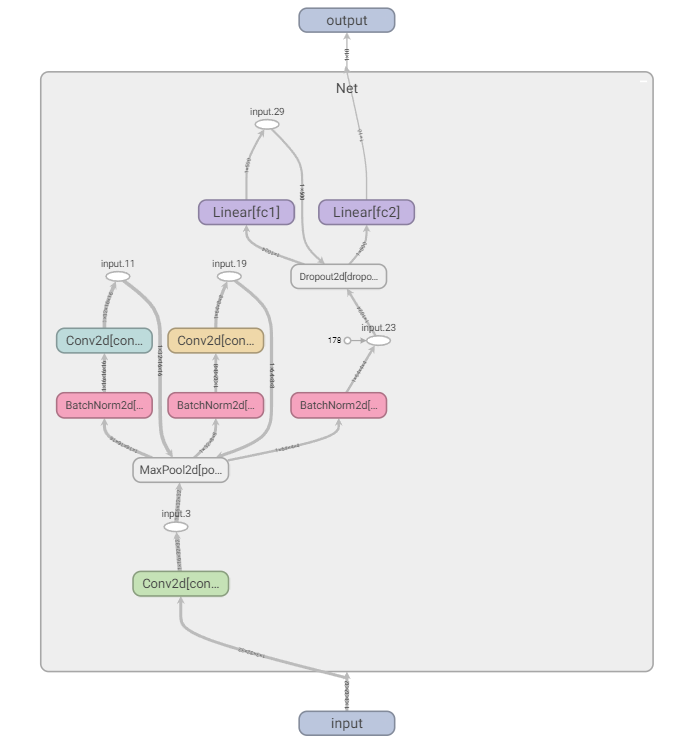
\includegraphics[width=18cm]{images/structure.png}
    \caption{实验模型流程概览}
\end{figure} 
\subsection{训练方法}
\paragraph{}我们使用梯度下降和反向传播的方法对模型进行训练.经过多次测试, 我们将学习率设置为0.005.梯度下降使用了torch的optim.SGD函数.
\begin{minted}{python}
optimizer = torch.optim.SGD(model.parameters(), lr=0.005)
\end{minted}
\paragraph{}训练过程如下:
\begin{minted}{python}
for epoch in range(1, n_epochs + 1):
    train_loss = 0.0
    model.train()
    for data, target in train_loader:
        data, target = data.cuda(), target.cuda()
        optimizer.zero_grad()
        output = model(data)
        loss = criterion(output, target)
        loss.backward()
        optimizer.step()
        train_loss += loss.item()*data.size(0)

    train_loss = train_loss/len(train_loader.sampler)
\end{minted}
\paragraph{}每轮训练后将在tensorboard中记录loss数据用于模型评估.训练轮次设置为100次.

\subsection{训练过程监控和可视化}
\paragraph{}为了更好地分析模型和优化参数,我们使用tensorboard记录中间参数(如分类准确率和loss)并做可视化.在每轮迭代后我们将训练集的loss记录在tensorboard中,每经过5轮迭代后我们分析测试集的分类准确率和loss并记录,这有利于我们分析参数设置和监控训练过程.
\paragraph{}相关代码示例如下,相关参数的可视化结果将在下节展示并分析.
\begin{minted}{python}
writer.add_scalar('Loss of Train Data',train_loss,epoch)
\end{minted}

\subsection{结果评估}
\paragraph{}我们使用测试集的分类准确率(包括平均分类准确率和各类图片的分类准确率)和loss来评估分类结果,具体代码如下,我们使用testAccuracy来分析最终分类结果和监控模型训练过程.
\begin{minted}{python}
def testAccuracy(loader, model):
    testLoss = 0.0
    classCorrect = list(0. for i in range(10))
    class_total = list(0. for i in range(10))
    model.eval()
    for data, target in loader:
        if train_on_gpu:
            data, target = data.cuda(), target.cuda()
        output = model(data)
        loss = criterion(output, target)
        testLoss += loss.item() * data.size(0)
        _, pred = torch.max(output, 1)
        correct_tensor = pred.eq(target.data.view_as(pred))
        correct = np.squeeze(correct_tensor.numpy()) if not train_on_gpu else np.squeeze(correct_tensor.cpu().numpy())
        for i in range(batch_size):
            label = target.data[i]
            classCorrect[label] += correct[i].item()
            class_total[label] += 1

    test_loss = testLoss / len(loader.dataset)
    writer.add_scalar('Loss of Test Data',
                      test_loss,
                      epoch)

    for i in range(10):
        className = classes[i]
        writer.add_scalar('Accuracy of ' + className+'/%',
                          100. * classCorrect[i] / class_total[i],
                          epoch)
    writer.add_scalar('Overall Accuracy/%',
                      100. * np.sum(classCorrect) / np.sum(class_total),
                      epoch)
\end{minted}

\section{实验过程和调参实验}
在实验过程中,我们设定了一系列的参数,包括训练学习率(lr)、dropout的比率、卷积层的层数、是否使用BN层。为了方便对比分析参数对实验的影响,我们设定了一组对照用的参数,为学习率lr=0.005,dropout比率0.4,卷积层3层,使用BN,将这种参数条件下的数据作为对照组。按照实验要求,每次实验都终止于第100次迭代。\par
\begin{definition}
对照组:学习率lr=0.005,dropout比率0.4,卷积层3层,使用BN,这是我们最终选择的最优参数设置
\end{definition}
注:由于我们的疏忽,考察训练集数据的loss时,计算了平均loss,而在考察测试集数据的loss时,没有将计算出的loss取平均值,所以两个loss的数值相差了100000倍,由于这个问题在撰写报告时才被发现,如果返工工作量会比较大,所以我们还是采用了原始数据,如果对读者造成困扰我们十分抱歉。
\subsection{训练过程}
为方便起见,我们在此使用对照组实验来展示实验的训练过程,由于训练过程的理论逻辑以及代码实现已经在本实验报告2.3模块中详细说明,所以在本模块中我们仅展示训练过程的数据变化过程。\par
我们利用tensorboard的图形化工具图形化了实验过程中loss、测试集准确率随epoch的变化过程。\par
对照组(lr=0.005,dropout比率0.4,卷积层3层,使用BN)的训练集loss、测试集loss、测试集准确率随epoch变化的曲线图分别如图2,图3,图4所示。\par
\begin{figure}[h]
\centering
\begin{minipage}[t]{0.3\textwidth} 
\centering
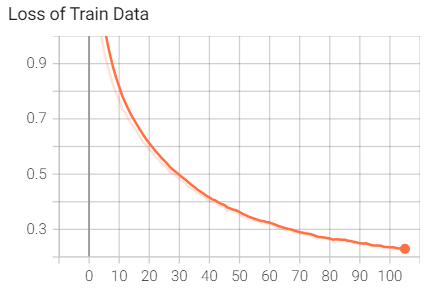
\includegraphics[scale=0.6]{images/train_loss.png}
\caption{训练集数据loss-epoch}
\end{minipage}
\begin{minipage}[t]{0.3\textwidth}%textwidth值小于0.25
\centering
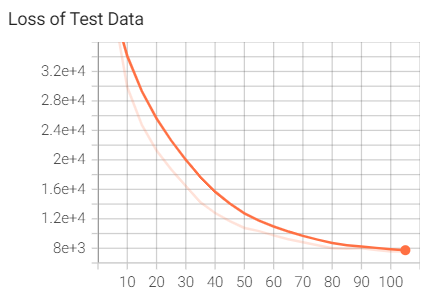
\includegraphics[scale=0.6]{images/test_loss.png}
\caption{测试集数据loss-epoch}
\end{minipage}
\begin{minipage}[t]{0.3\textwidth}%textwidth值小于0.25
\centering
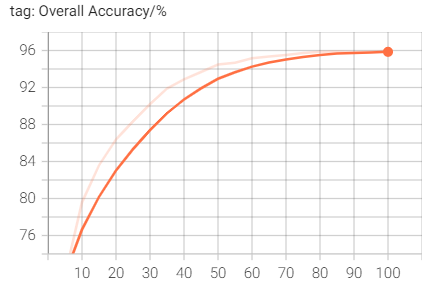
\includegraphics[scale=0.6]{images/accuracy.png}
\caption{测试集accuracy-epoch}
\end{minipage}
\end{figure}
可以看出变化趋势,训练过程中测试集和训练集loss都是呈先快速下降,后缓慢下降,最后趋于收敛的趋势,而测试集的准确率则呈先快速上升,后缓慢上升,最后趋于收敛的趋势。这组实验在训练过程中没有出现过拟合。
\subsection{调参实验及分析比较}
在本实验中,我们对上述四种参数训练学习率(lr)、dropout的比率、卷积层的层数、是否使用BN进行了调整,分析比较了调参后模型和对照组模型的loss、准确率以及其变化趋势,提出了一些我们的看法。\par
\subsubsection{学习率对训练过程和结果的影响}
在其他三种参数保持和对照组不变时,更改学习率learning rate的值。
将参数学习率lr改为0.003。测试集准确率变化趋势如图5所示。\par
\begin{figure}[h]
\centering
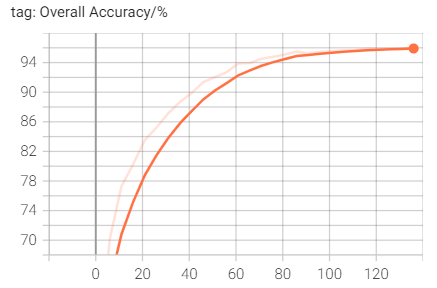
\includegraphics[scale=0.6]{images/lr003.png}
\caption{学习率为0.003时的测试集准确率趋势曲线}
\end{figure}
为了完整地展示测试集准确率的变化规律,我们将最大epoch设置成了130,可以看到,当把学习率调低时,在epoch=100时准确率曲线并未收敛,而在epoch接近120时才收敛,训练过程中准确率收敛需要的迭代次数会增加。同时由于epoch=100时仍未收敛,此时的训练集准确率为95.54\%,低于对照组。\par
\begin{observation}
学习率过低会影响模型在训练时的收敛速度,且模型最高准确率提升不明显.\par
\end{observation}
下面将参数学习率lr改为0.008.\par
\begin{figure}[H]
\centering
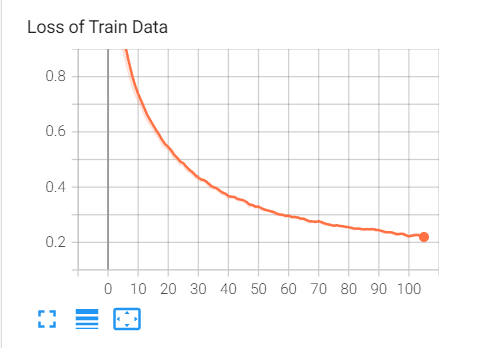
\includegraphics[scale=0.6]{images/loss_train_lr008.png}
\caption{学习率为0.008时的测试集loss趋势曲线}
\end{figure}
可以看到,在训练过程中train loss经常起伏波动,说明学习率过高会影响训练的稳定性,导致训练过程难以较快收敛。epoch=100时的训练集准确率为96.02\%。
\begin{observation}
学习率过高会影响训练过程的稳定性,影响模型收敛速度,使模型很难较快收敛到局部最优解.\par
\end{observation}

\subsubsection{dropout层的有无对训练过程和结果的影响}
在本小节中,我们保持其他三种参数保持和对照组相同,更改dropout的比率。
将dropout比率改为0.5。测试集准确率变化趋势如下图所示。\par
\begin{figure}[H]
\centering
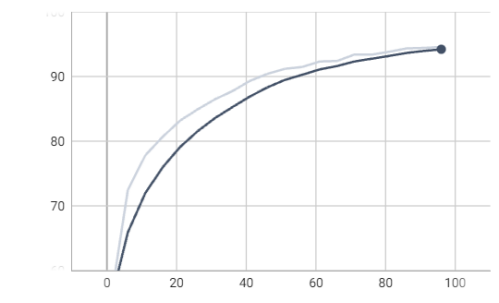
\includegraphics[scale=0.6]{images/dr05.png}
\caption{dropout为0.5时的测试集准确率趋势曲线}
\end{figure}
可以看到在epoch=100时并未收敛,说明dropout的比率过大时,需要更长的训练过程来完成训练。在epoch=100时,测试集准确率为94.54\%,低于对照组。\par
\begin{observation}
dropout率过高会影响模型收敛速度和准确率.\par
\end{observation}

我们还测试了没有dropout层的情况下的情况。\par
\begin{figure}[H]
  \centering
  \subfigure[测试集loss]{
    \label{fig:subfig:onefunction} 
    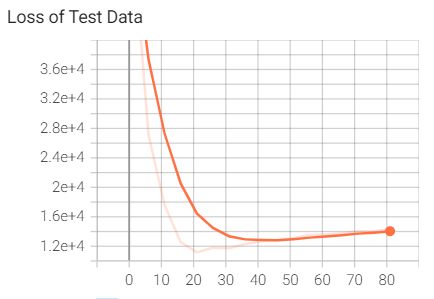
\includegraphics[scale=0.5]{images/nodr_test.png}}
  \hspace{0.5in} % 两图片之间的距离
  \subfigure[训练集loss]{
    \label{fig:subfig:twofunction} 
    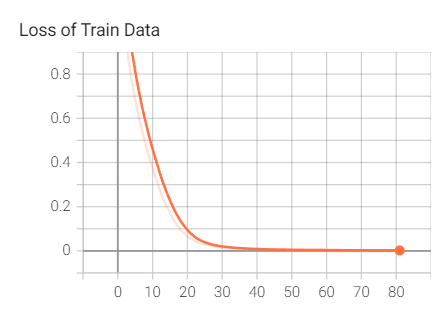
\includegraphics[scale=0.5]{images/nodr_train.png}}
  \caption{没有dropoout层情况下训练情况}
  \label{fig:twopicture} 
\end{figure}
可以看到虽然测试集loss逐渐收敛,但是测试集的loss在epoch=30附近出现了不减反增的情况,说明训练过程中出现了过拟合现象(模型对训练集的个性化特征过于重视,导致模型无法学习到数据的普遍规律,从而导致测试集的loss上升),说明dropout可以有效防止过拟合。
\begin{observation}
dropout率过低或没有dropout层会导致模型训练容易出现过拟合.\par
\end{observation}

\subsubsection{卷积层个数对训练过程和结果的影响}
在本节中,我们在其他三种参数保持和对照组相同的条件下,更改卷积层的层数。\par
将卷积层改为2层,发现各种评估指标的趋势没有明显变化,但epoch=100时测试集准确率为95.45\%,低于卷积层为3层时的准确率,同时每轮训练所需的时间减少,但达到收敛所需的训练轮次增加。\par
将卷积层改为4层,发现模型训练过程中出现一定的过拟合现象,epoch=100时测试集准确率为95.31\%,低于卷积层为3层时的准确率,同时每轮训练所需时间增加。
\begin{observation}
卷积层过少时模型参数过于简单,无法提取到数据的全部特征,分类准确率低;卷积层过多时模型参数过于复杂,容易出现过拟合,也会影响分类准确率. \paragraph{}同时卷积层较少时每轮训练所需时间短,但达到收敛所需的迭代次数多,卷积层较多时每轮训练所需时间长,但达到收敛所需的迭代次数少.\par
\end{observation}

\subsubsection{BN层对训练过程和结果的影响}
在本节中,我们在其他三种参数保持和对照组相同的条件下,去掉BN层。\par
\begin{figure}[H]
\centering
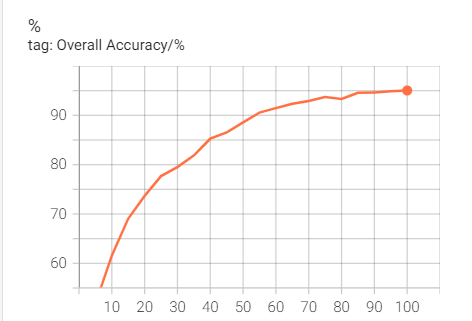
\includegraphics[scale=0.6]{images/acc_no_bn.png}
\caption{去掉BN之后的测试集准确率趋势曲线}
\end{figure}
可以看到测试集准确率在训练过程中产生了较大起伏,说明BN层有助于稳定训练过程。此外,发现去掉BN之后程序的运行时间比去掉BN之前长,说明BN也可以有效地缩短训练时间。
\begin{observation}
BN层有助于稳定训练过程,并缩短训练时间
\end{observation}

\section{实验结果和最高准确率}
\subsection{实验得到的最佳参数设置}
\paragraph{}经过实验,我们发现采用学习率lr=0.005,dropout比率0.4,卷积层为3层,使用BN层的参数设置时的模型分类准确率最高.
\subsection{最高准确率}
在epoch=100时,使用上述模型得到的测试集数据分类准确率为96.02\%,不限定训练次数的模型最高分类准确率也为96.02\%,因为100次迭代后模型训练达到收敛.
\paragraph{}下面是使用上述模型100次迭代后各类图像的分类准确率. \paragraph{}我们发现dog和cat的分类准确率明显低于其他类别,这可能是由于dog和cat长相上相似度较高造成的,在之后的改进模型中,我们可以根据dog和cat的特征对模型做针对性改进来提高dog和cat的分类准确率.
\paragraph{}此外,各类图像分类准确率变化的趋势并不完全相同,有些类别的图像的分类准确率在训练结束时尚未达到收敛(如cat),但是有些类别的图像的分类准确率在训练结束时已经在达到峰值后下降(如airplane,可能是过拟合引起的),最高的平均分类准确率并不意味着所有图像的分类准确率都达到了最高,这也为我们改进模型提供了思路.
\begin{table}[h!]
  \begin{center}
    \caption{各类图像分类准确率}
    \begin{tabular}{l|c|r}
      \textbf{类别名} & \textbf{分类准确率}\\
      \hline
      airplane & 96.8\% \\
      automobile & 98.5\% \\
      bird & 93.52\% \\
      cat & 91.92\% \\
      deer & 95.5\% \\
      dog & 93.52\% \\
      frog & 97.78\% \\
      horse & 96.94\% \\
      ship & 98.34\% \\
      truck & 97.52\% \\
      average & 96.03\% \\

    \end{tabular}
  \end{center}
\end{table}

\section{实验总结}
在本次实验中,我们调研并学习了使用CNN实现图像分类的知识,完成了训练和测试的代码,并调整和测试了了一些参数,对结果进行了比较分析。在调参、比较、分析的过程中,我们总结了一些规律和结论,如
\begin{itemize}
    \item 合适的学习率对于模型和训练十分重要,学习率过低时模型收敛缓慢,学习率过高时模型训练不稳定并很难达到局部最优解.
    \item dropout可以有效防止过拟合,但dropout比例过大会导致模型underfit从而影响模型分类准确率.
    \item BN可以有效稳定训练过程并加快训练速度.
    \item 搭建CNN模型时为了取得最高分类准确率应该不断增加卷积层数目直到出现过拟合为止,但是卷积层过多也会导致训练速度缓慢,某些情况下需要平衡这两者之间的关系.
    \item 在CNN模型中前几个卷积层应该尽量宽以便充分提取数据特征,后几个卷积层应该逐渐变窄以便充分组合各类特征.
\end{itemize}
\paragraph{}本模型还存在很多不足之处,可以在以后加以改进,如
\begin{itemize}
    \item 本模型在每层卷积后都添加了BN,但是一些资料显示,在前几个卷积层后无需添加BN,且在前几个卷积层添加BN可能会影响样本特征的充分提取和模型的分类准确率.
    \item 在平均分类准确率达到最大时一些类别的分类准确率尚未达到收敛,而一部分类别的分类准确率已经出现了过拟合,这可能影响模型在不同场景下的应用,可以针对不同样本的特征学习情况对模型做针对性的改进.
    \item 部分特征相近的类别的图像的分类准确率显著较低(如dog和cat),可以针对这类情况做针对性的改进.
    \item 可以充分利用现有硬件的并行计算能力对训练做并行化改进来加快训练速度,此外,可以利用现有的分布式计算框架对模型做改进.
\end{itemize}

本次实验帮助我们巩固了知识,培养了调参、分析的能力,使我们受益匪浅。

\nocite{*}
\bibliographystyle{plain}
\bibliography{
ref-1.bib,
ref-2.bib,
ref-3.bib,
ref-4.bib,
ref-5.bib,
}
\end{document}
